\documentclass[fleqn,10pt]{wlscirep}
\usepackage[utf8]{inputenc}
\usepackage[T1]{fontenc}
\usepackage{graphicx}
\usepackage{tablefootnote}
\usepackage{xr}

\makeatletter
\newcommand*{\addFileDependency}[1]{% argument=file name and extension
  \typeout{(#1)}
  \@addtofilelist{#1}
  \IfFileExists{#1}{}{\typeout{No file #1.}}
}
\makeatother


\newcommand*{\myexternaldocument}[1]{%
    \externaldocument{#1}%
    \addFileDependency{#1.tex}%
    \addFileDependency{#1.aux}%
}

\myexternaldocument{SI}

\title{NMRlipids Databank: Making data-driven analyses of membrane properties accessible for all}
%Overlay Databank of Lipid Membrane Simulations Arising from Open Collaboration}

\author[1]{Anne Kiirikki}
\author[2]{...}
\author[1,*]{O. H. Samuli Ollila}
%\author[1,2,+]{Christine Author}
%\author[2,+]{Derek Author}
\affil[1]{University of Helsinki, Institute of Biotechonology, Helsinki, Finland}
\affil[2]{Affiliation, department, city, postcode, country}

\affil[*]{samuli.ollila@helsinki.fi}

%\affil[+]{these authors contributed equally to this work}

%\keywords{Keyword1, Keyword2, Keyword3}

\begin{abstract}
We present a databank of lipid bilayer simulations from the NMRlipids open collaboration project.
\end{abstract}
\begin{document}

\flushbottom
\maketitle
% * <john.hammersley@gmail.com> 2015-02-09T12:07:31.197Z:
%
%  Click the title above to edit the author information and abstract
%
\thispagestyle{empty}

%\noindent Please note: Abbreviations should be introduced at the first mention in the main text – no abbreviations lists. Suggested structure of main text (not enforced) is provided below.

\section{Introduction}

%The demand for sharing and reusing of MD simulation data is increasing, but practical solution remains unclear due to unsolved issues in data storage and indexing.

Cellular membranes are composed of hundreds of different types of lipid molecules which regulate membrane properties, morphology and biological functions~\cite{vanmeer08}. Membrane lipid composition can be also related to diseases, such as cancer and neurodegenerative disorders, and potential therapeutics that affect membrane compositions have been proposed~\cite{torres21}. However, membrane-containing systems are often difficult to study experimentally because the membranes are in a disordered fluid state under biological conditions and sample preparation can be arduous due to the complicated phase behaviour and rich interactions between lipids and other biomolecules. For those reasons, the detailed connections between lipid interactions and biological functions taking place in or around membranes are still poorly understood.
%why such variety of lipids is needed and how their. 
Molecular dynamics (MD) simulations have been particularly useful in understanding membrane systems, yet their accuracy is often compromised by the quality of model parameters, methodological inadequacy, and other artefacts~\cite{antila22b,gupta22}. 
%While MD simulations of systems with few biomolecules continue having major contributions in our understanding on biology and drug design, 
On the  other hand, the accuracy of models is becoming increasingly important as the scale (in both size and time) of the systems studied continuously increases 
%researches are progressing from the simulations of 
%now searching new avenues by building models not only 
from the level of individual molecules to models of whole cells or organelles using interdisciplinary approaches~\cite{johnson15,thornburg22,gupta22}. Such systems exhibit complex emergent behaviour making inaccuracies more difficult to detect and accumulation of even modest errors may have major effects the conclusions.

In contrast to experimental structural biology, where standard protocols to share and quality evaluate the resolved structures are established in the PDB databank~\cite{montelione13}, the equivalent best practices are yet to be defined for MD simulations. The importance of such approaches is widely recognized~\cite{feig99,tai04,silva06,abraham19,hildebrand19,hospital20,abriata20,espigares20} and solutions for sharing data are emerging for proteins in solution~\cite{meyer10,kamp10}, proteins in membranes~\cite{newport19,espigares20,leston22}, nucleic acids~\cite{hospital16}, cyclodextrins~\cite{mixcoha16}, and arbitrary biomolecules~\cite{bekker20}. However,
%The relevance of quality evaluation of simulation trajectories in databanks regarding technical details of simulations and accuracy of the underlying physical description of the system (force field) has become evident~\cite{tai04,meyer10,hospital20} and such 
a streamlined workflow with automatic quality evaluation~\cite{meyer10,hospital16} and programmatic access is still rare. 
%However, straightforward quality comparisons between individual simulations or force fields within these databanks remain challenging. 
Therefore, tools for automatic quality evaluation of membrane simulations or training sets for machine learning models of membrane-containing systems are not yet available. 

%Applications of MD simulations in understanding biomolecular behaviour are steadily increasing, but protocols for quality evaluation and sharing simulation data fall behind the ones in more elaborated fields, such as structural biology. Development of such protocols has been limited by practical challenges, such as lack of universally defined quality measures for MD simulations, incompatible naming conventions in different models and simulation softwares, and high technical requirements for hardware to share large trajectories from MD simulations, as well as incentives for scientist to evaluate and share their MD simulation data. 


Here we present the NMRlipids databank, a community-driven open access databank with programmatic access containing atomistic resolution MD simulations of lipid bilayers. The programmatic access enables various data-driven approaches, providing new tools for researchers in a wide range of fields covering academia and industry from cell membrane biology to lipid nanoparticle formulations, data-driven computational chemistry, and machine learning. Here, we demonstrate how data-driven analysis of water anisotropic diffusion in membrane systems from the NMRlipids databank can extend the scope of MD simulations to MRI imaging and pharmacokinetics as well as how the NMRlipids databank can be utilized to analyse rare phenomena that are beyond the scope of standard MD simulation investigations. Furthermore, we perform automatic quality evaluation of membrane simulations, which guides the selection of best models for specific applications and the improvement of simulation parameters and methodology.
%The practical relevance of the NMRlipids databank is exemplified by automatic quality evaluation and ranking of large amount of MD simulation data, 

While the NMRlipids databank currently contains only bilayer systems, it can readily be expanded to contain other molecules than lipids, such as disordered proteins or sugars. 
%a solution for lipid bilayers based on overlay databank structure illustrated in Fig.~\ref{fig:overlay}.  
The combination of an overlay databank structure and a community-wide open collaboration used here has been applied successfully when building databanks in other fields,  
%is developed here to solve the practical challenges in generating databanks of MD simulation data enabling flexible analyses over large sets of simulation data, but it can be  potentially used for wide range of situations. 
particularly when storage of raw data requires significant resources, best practices in the field are not defined, and incentives to share data do not exist.
%overlay databank approach lowers the barrier to start without compromizing the long term stability or scalability.
Thus, the approach has already proven itself most useful in enabling data-driven and machine learning applications in new fields. 



%The Introduction section, of referenced text\cite{Figueredo:2009dg} expands on the background of the work (some overlap with the Abstract is acceptable). The introduction should not include subheadings.

\section{Results}

%Up to three levels of \textbf{subheading} are permitted. Subheadings should not be numbered.
\subsection{Programmatic access to MD simulation data of membranes composed of most common biologically abundant lipids}
NMRlipids databank is a community-driven databank containing atomistic MD simulations of biologically relevant lipid membranes emerging from the NMRlipids open collaboration~\cite{botan15,ollila16,catte16,antila19,bacle21}. Nearly a thousand simulation trajectories with the total length approaching half a millisecond can be accessed programmatically using the Python application programming interface (API) or a graphical user interface (GUI) (\url{http://www.databank.nmrlipids.fi/}). 
%NMRlipids databank is the only databank of MD simulations with open programmatic access to its content enabling fully flexible analyses of its content. 
Following the FAIR principles~\cite{wilkinson16} and NMRlipids project protocol, not only the content and computer programs related to the databank, but also the entire construction process of the databank, are open access~\cite{botan15}. 
%The NMRlipids databank will be always open for data and other contributions.

Currently available single component lipid membranes and binary mixtures in the NMRlipids databank are illustrated in Fig.~\ref{fig:overlay}D. While these comprise the majority of available trajectories, mixtures with up to five lipid types are available. The distribution of available simulations containing a specific lipid is shown in Fig.~\ref{fig:overlay}C. This roughly resembles the biological abundance of different lipid types with phosphatidylcholine (PC) being the most common followed by cholesterol, phosphatidylethanolamine (PE), phosphatidylserine (PS), phosphatidylglycerol (PG), phosphatidylinositol (PI), and other lipids depending on organism and organelle~\cite{vanmeer08}. The force fields used in the simulations cover all the essential parameters commonly used in lipid simulations, ranging from highly popular CHARMM36 parameters to united atom and polarizable force fields. Therefore, the averages calculated over the databank can be considered as mean predictions from available lipid models for an average cell membrane.
%Currently the databank is composed of approximately 500 trajectories with the total length of approximately 231 microseconds of which most are contributed for the previous publications from the NMRlipids open collaboration~\cite{botan15,catte16,antila19,bacle21}. The distribution of lipids, force fields, length of the trjajectories and available binary mixtures are shown in Fig.~\ref{fig:overlay}. 

The efficient upcycling of large MD simulation trajectories in the NMRlipids databank is enabled by the overlay structure illustrated in Fig.~\ref{fig:overlay}A. Raw simulation data in the {\it data layer} can be stored in any publicly available location with long term stability and permanent links to the data (e.g., digital object identifiers (DOIs)). The {\it Databank layer} is the core of the databank containing all the relevant information about the simulations, including links to the raw data, relevant metadata describing the systems, universal naming conventions for the lipids and their atoms, computer programs to create and analyse the entries, basic properties calculated from all simulations (area per lipid, C-H bond order parameters, X-ray scattering form factors and membrane thickness), and quality evaluation of simulations against experimental data. In practise, this information is stored is the git repository which is currently available at~\url{https://github.com/NMRLipids/Databank}. The {\it application layer} contains outputs from the databank, such as graphical user interface (\url{http://www.databank.nmrlipids.fi/}), and results from analyses described in sections below. A more detailed description on the NMRlipids databank structure is available the supplementary information. 

%are enabled by the 
%The databank can be used in layer 3 by accessing the raw data and information stored in the databank by employing the universal naming conventions for atoms, molecules and simulation details. The applications can be linked to the core databank (layer 2) without actually including them, thereby enabling flexible extension of the data without compromising the simplicity and lightness of the core databank.

\begin{figure}
    \centering
    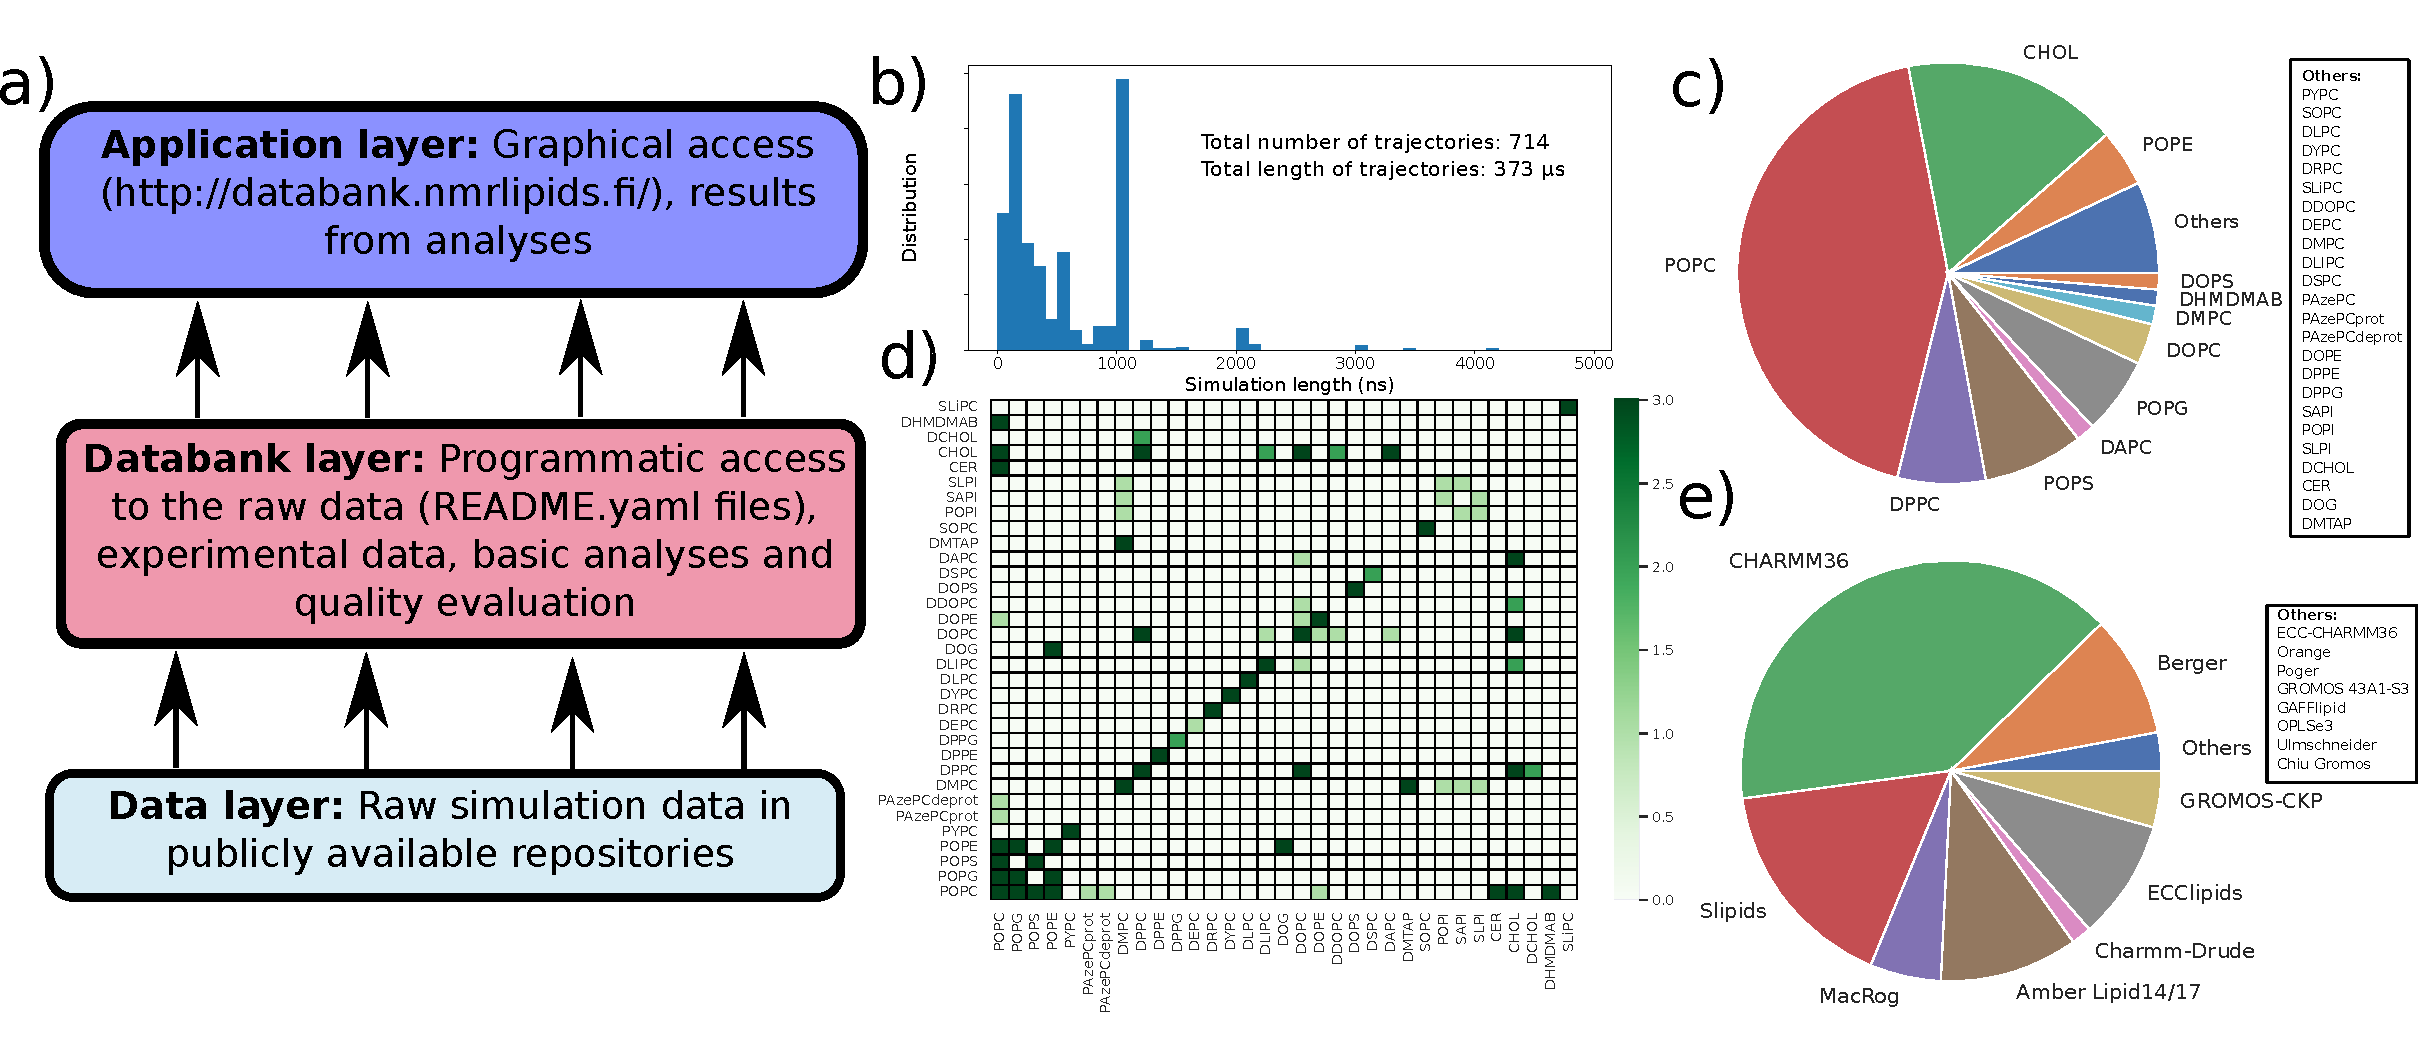
\includegraphics[width = 180mm]{Figures/overlay2.pdf}
    \caption{a) Structure of an overlay databank. 
    %Raw data is available from a publicly accessible repository (layer 1).
    %The core of the databank contains information on the location of the raw data and indexing of molecular %compositions and simulation details described with universal naming conventions (layer 2).
    %The content of databank can be viewed and analysed using external programs that automatically read the information and data from layers 1 and 2 (layer 3). Examples of such applications are the GitHub repository generating the results presented in this work and the graphical access to the databank.
    More detailed structure of the layer 2 in the NMRlipids databank is illustrated in Fig.~\ref{DatabankStructure} in the SI.
    b) Distribution of the lengths of the trajectories, total number of trajectories and total lenght of the simulations in the NMRlipids databank.
    c) Distribution of lipids present in the trajectories in the NMRlipids databank. Lipids occuring in five or less simulations ('others') are listed in the right. 
    d) Currently available binary mixtures in the NMRlipids databank. 
    e) Distribution of force fields in the simulations in the NMRlipids databank.
    }
    \label{fig:overlay}
\end{figure}


\subsection{Selection of best simulation parameters for applications using the NMRlipids databank}
%Quality of membrane simulations with different force fields have been evaluated against experimental data during parameterization and in separate comparison studies~\cite{botan15,ollila16,catte16,pluhackova16,perez17,leonard19,??}, but the lack of universal quality measure for membrane simulations complicates the estimations of reliability of simulations. 
Understanding the accuracy of used force field parameters is crucial when assessing the reliability and significance MD simulation results. However, the lack of universal quality measures for MD simulations and the complicated landscape of force field quality for membranes hamper the applicability such simulations, resulting in substantial controversies~\cite{antila22b}. For example, previous quality evaluations of membrane simulations have concluded that CHARMM36 parameters give the best description for lipid headgroup conformational ensembles~\cite{bacle21}, GROMOS-CKP parameters best capture the membrane packing in POPS bilayers~\cite{antila22b}, and that OPLS3e parameters overcome CHARMM36 in structural quality for POPC but predicts overestimated ion binding~\cite{kurki22}. 
%, thereby being a major obstacle in many applications of membrane MD simulations. 
To enable the navigation in this complex force field milieu, we here define quantitative quality measures that can be used to rapidly find the best available parameters for a specific application or to guide the development of improved force fields. For detailed definitions of quality measures, see the supplementary information.

\begin{figure}[!t]
    \centering
    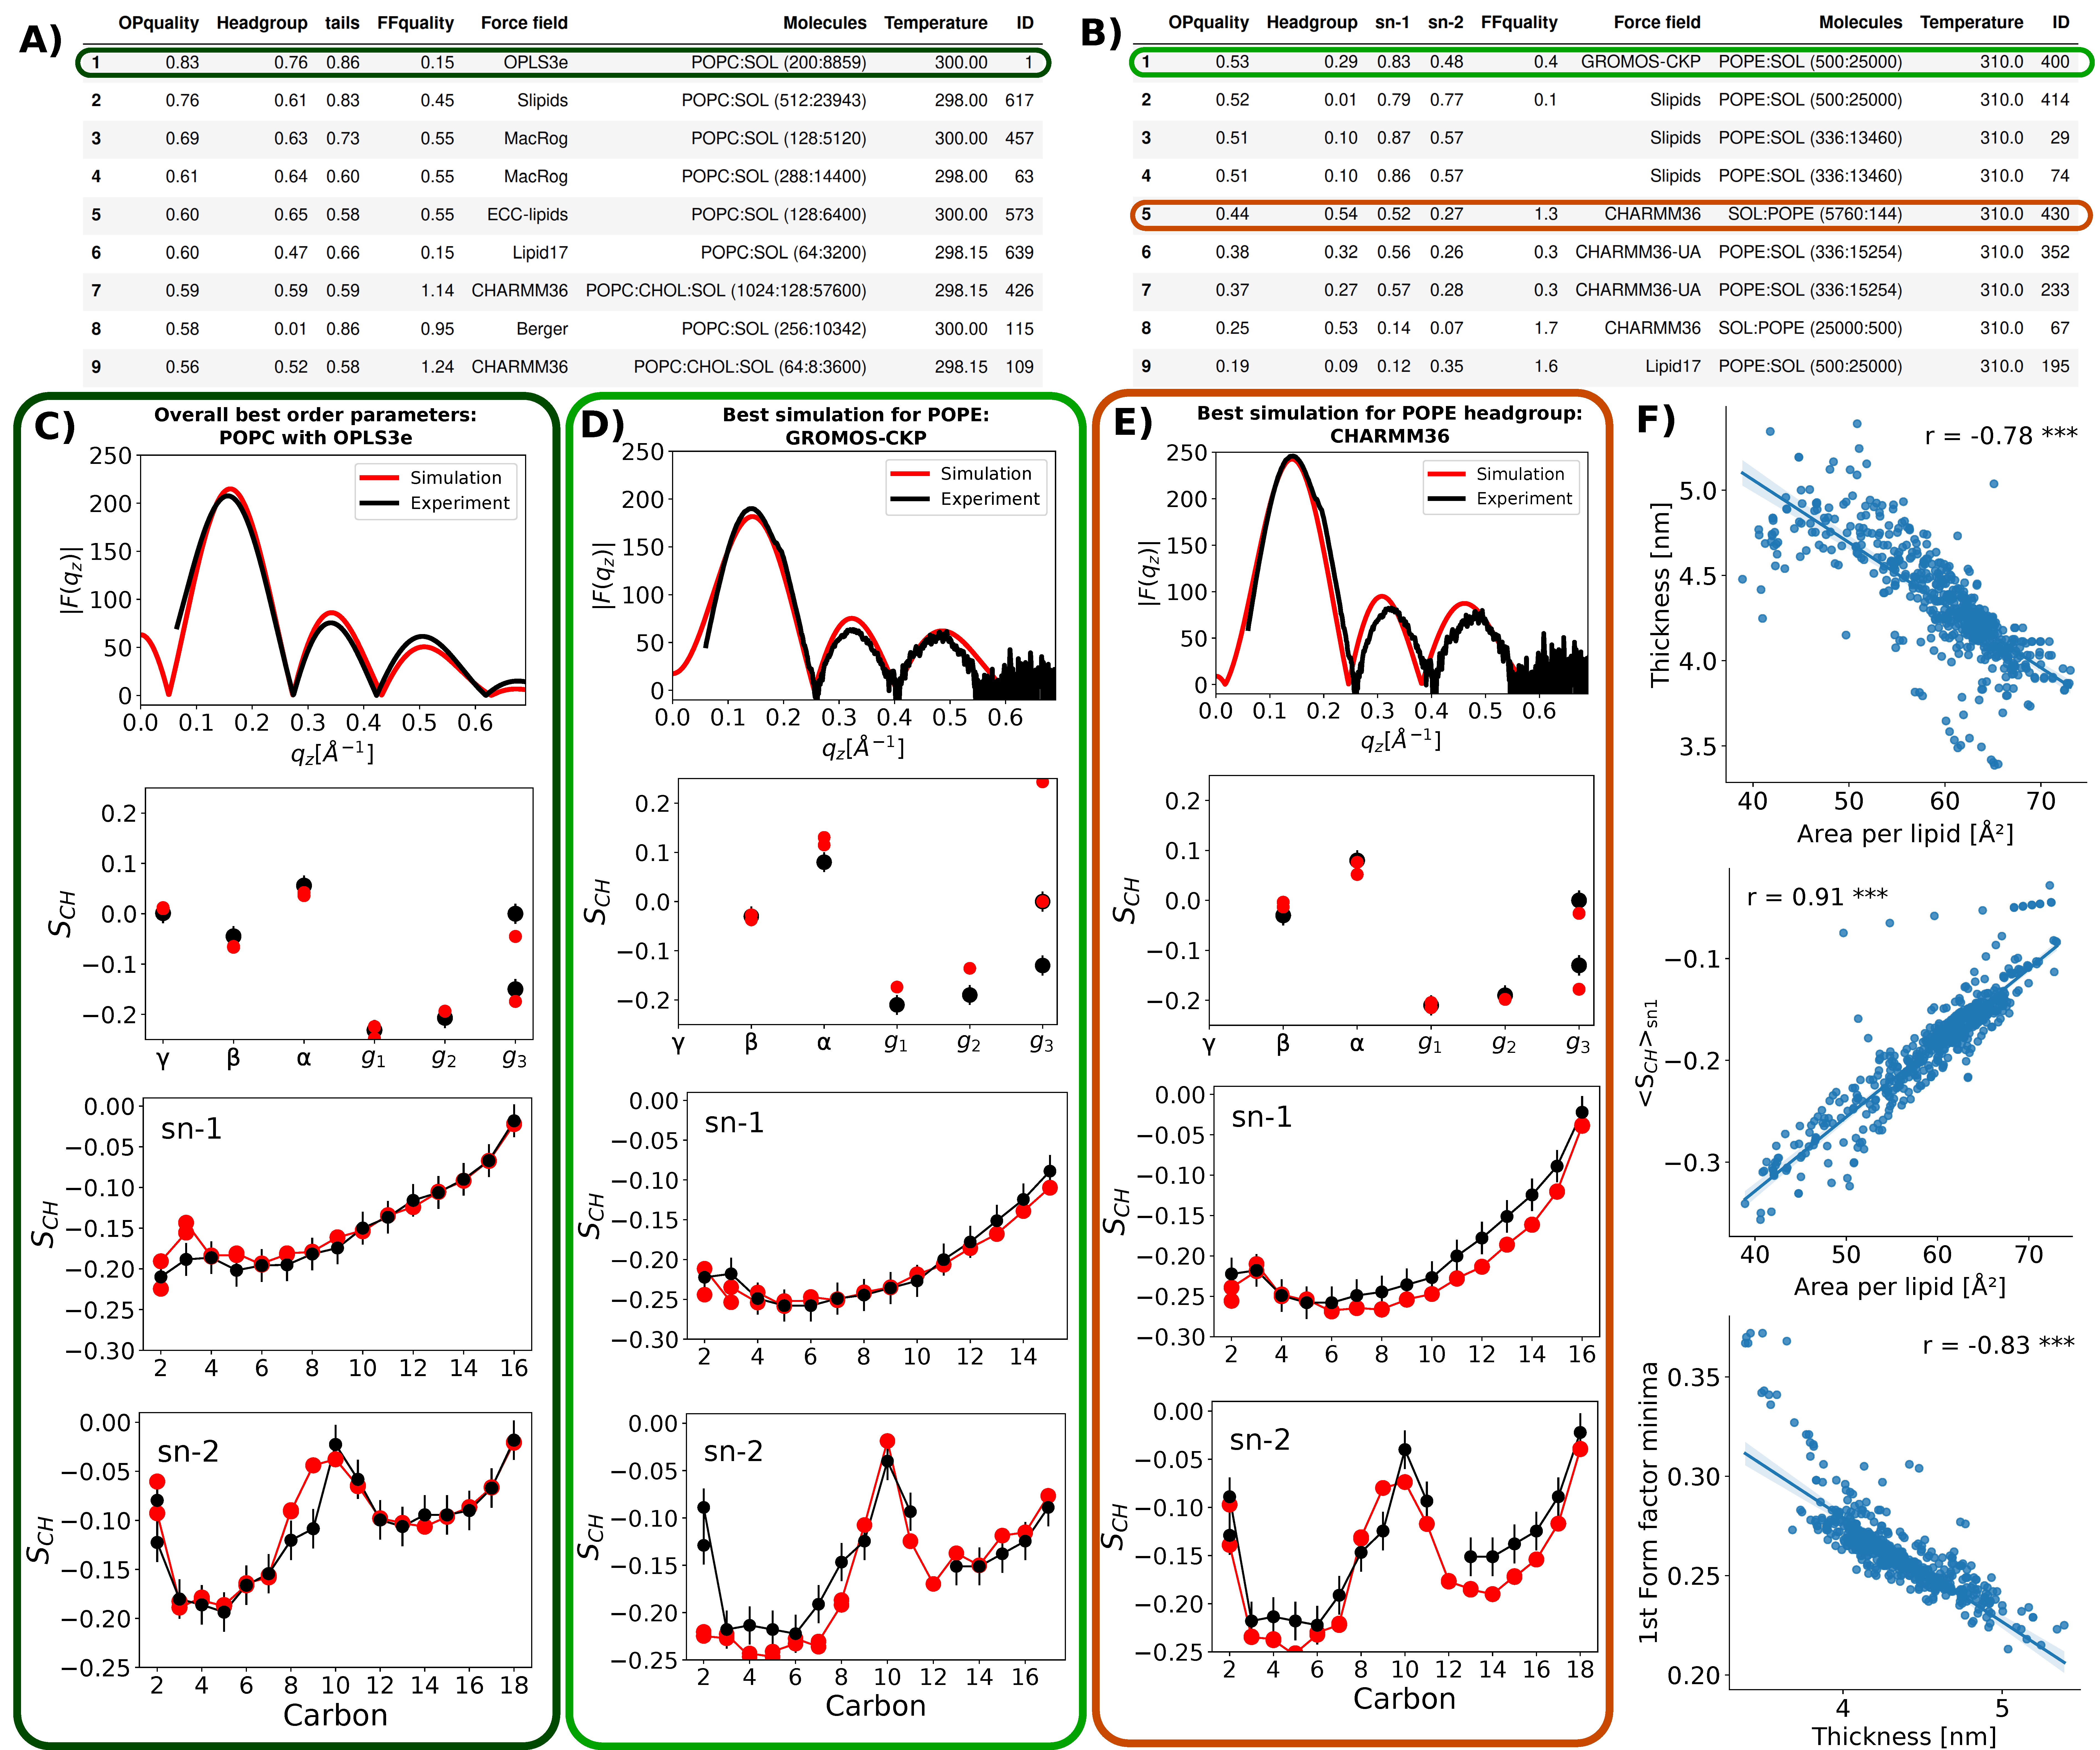
\includegraphics[width=180mm]{Figures/quality3.pdf}
    \caption{ A) Best simulations ranked based on overall order parameter quality.
    B) Best simulations ranked based on the overall order parameter quality of POPE lipid. 
    C)-E) Evaluation against experimental data exemplified for a simulation with the best overall order parameter quality (C), the best quality for POPE lipid (D), and the headgroup quality for POPE (E).
    F) Scatter plots and Pearson correlation coefficients for the membrane area per lipid, thickness, first minima of x-ray scattering form factor and average order parameter of the {\it sn}-1 acyl chain extracted from the NMRlipids databank. 
    All correlation coefficients have p-value below 0.001. For more correlations see Fig.~\ref{fig:QualityCorrelationsSI}.
    }
    \label{fig:quality}
\end{figure}


Ranking of all simulations with the highest scores based on evaluation against C-H bond order parameters from NMR experiments is shown in Fig.~\ref{fig:quality} A and ranking of best POPE lipid bilayer simulations in Fig.~\ref{fig:quality} B. Direct comparisons with experiments for selected simulations are shown in Figs.~\ref{fig:quality} C-D. C-H bond order parameters are sensitive to conformational ensembles of individual lipid molecules~\cite{ollila16} while also correlating well with the membrane thickness and lateral packing as shown in Fig.~\ref{fig:quality} F. This is complemented by comparing the absolute values of X-ray scattering form factors between simulations and experiments that are related to the overall membrane dimensions via the electron density profile. In particular, the location of minima in these form factors are correlated with the membrane dimensions as shown in Figs.~\ref{fig:quality} F,~\ref{fig:QualityCorrelationsSI}, and~\ref{fig:sizedependence}.

%best simulation, POPC with OPLS3e, is shown in
%based on C-H bond order parameters from NMR experiments and x-ray scattering form factors that enable the rapid quality evaluation of membrane MD simulations in the NMRlipids databank. 

%Order parameters and scattering form factors are robust experimental measurables that can be directly connected to the simulation data~\cite{ollila16}. 

%NMRlipids databank contains also experimental order parameter and x-ray form factor data that is connected to corresponding  simulations in order to define the simulation qualities and rank them to select the suitable simulation models for particular applications. 

%Fig.~\ref{fig:quality} C, where discrepancies with experiments are observed only for the third carbon in the $\it{sn}$-1 chain, and carbons 8 and 9 close to the double bond in $\it{sn}$-2 chain. The best overall quality for POPE is found in GROMOS-CKP simulation, for which the direct comparison in Fig.~\ref{fig:quality} D show minor differences in acyl chains, but major discrepancies in glycerol backbone and in the first carbon of $\it{sn}$-2 chain. These parts are better described for POPE by CHARMM36 parameters (direct comparison shown in Fig.~\ref{fig:quality} E), but its overall quality suffers from the overestimated order in acyl chains. 


%\subsection{Finding the best models for PC and PE lipid mixtures}
The power of the NMRlipids databank in selecting the best simulation parameters for a specific application is demonstrated for mixtures of PE and PC lipids in Fig.~\ref{fig:POPCPOPEapls}, showing areas per lipid from available POPC and POPE bilayer simulations in the databank from different force fields at 310\,K. Predictions from different force fields deviate significantly in terms of absolute values and the slope of decrease upon addition of POPE. Because the area per lipid correlates with the average order parameter of the $\it{sn}$-1 chain (Fig.~\ref{fig:quality} F), simulations with the best predictions for area per lipids can be selected based on order parameter quality evaluation. Quality evaluation in Fig.~\ref{fig:quality} and direct comparison in Fig.~\ref{fig:POPC_POPE_dataSI} reveal that Slipids ranks 1st for POPC with a clear advantage to the others, and 2nd for POPE with only marginally lower quality score than GROMOS-CKP and is therefore the best avilable choice for studies where packing effects of PE lipids are important. 
%The direct comparison with experiments in Fig.~\ref{fig:POPC_POPE_dataSI} in the supplementary information reveals that 
Simulations with CHARMM36 and GROMOS-CKP predict overly packed bilayer for POPC (overestimated order in Fig.~\ref{fig:POPC_POPE_dataSI}), while the area per lipid for POPC is overstimated in Lipid17. For POPE, 
%order parameters in  Slipids and GROMOS-CKP are close to experiments suggesting that their are per lipids are most reasonable, while
CHARMM36 and Lipid17 predict membranes that are too packed. 


In conclusion, 
%the quality evaluation based on the NMRlipids databank suggests that the Slipids parameters would give the most reliable description for membrane packing of POPC:POPE mixtures. Slipids was a relatively good model also for POPC:POPS mixtures in similar comparisons utilizing the preliminary version of the NMRlipids databank~\cite{antila22b}, although charged membranes are more complicated as the counterion binding affinity plays a significant role in membrane packing~\cite{antila19}. On the other hand, CHARMM36 overcomes Slipids when the focus is on conformational ensembles of headgroups  in different types of lipids because the accuracy of glycerol backbone is low in Slipids~\cite{bacle21}. Altogether, these examples demonstrate how 
the automatic quality evaluation in the NMRlipids databank enables rapid exploration and selection of the best simulation parameters for specific applications without extensive and tedious manual force field evaluation. This possibility will promote more reliable simulation results for wide range of applications, support force field development and parametrization of coarse grained force fields against the best atomistic MD simulations. The automatically extracted quantitative quality measures will be particularly useful to guide automatic parametrization procedures.

\begin{figure}[tbp]
    \centering
    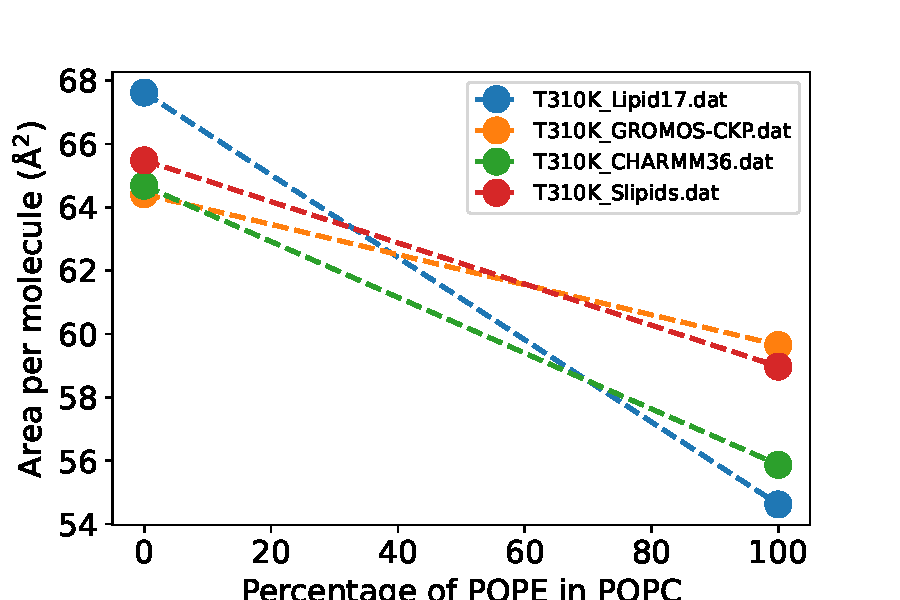
\includegraphics[width=88mm]{Figures/APL.pdf}
    \caption{Differences in area per lipids of POPC and POPE bilayers between different force fields.  
    }
    \label{fig:POPCPOPEapls}
\end{figure}


%On the other hand, the first form factor minima is correlated stronger with membrane thickness (Fig.~\ref{fig:quality} C) than with the area per lipid (Fig.~\ref{fig:QualityCorrelationsSI}). 
%Scatter plots and Pearson correlation coefficients in Fig.~\ref{fig:quality} C reveal strong correlation between membrane area per lipid and thickness.


%Understanding such complex picture of lipid bilayer MD simulation quality would not be possible without automatic quality evaluation of large sets of simulations enabled by the NMRlipids databank.

%The power of NMRlipids quality metrics in selecting the best model for particular application is demontrated in Fig.~\ref{fig:quality} c) where the area per lipids of POPC:POPE mixtures from different force fields are shown and quality of POPE simulation in different force fields are evaluated. 



 %This is demonstrated in Fig.~\ref{fig:quality} a) showing correlations between membrane lateral density (area per lipid), thickness, minima of form factor and acyl chain order analyzed from all apporimately 500 trajectories in the NMRlipids databank. Membrane area per lipid has negative correlations with membrane order and thickness with Pearson coefficient of -0.78 and -0.49, respectively, because decreased area leads to more ordered, tightly packed and stretched acyl chains leading to thicker membranes. On the other hand, locations of form factor minima have positive correlation with the membrane area and negative correlation with the thickness. In conclusion, both x-ray scattering form factors and acyl chain order parameters from NMR are on average good proxies for membrane packing and thickness, while NMR order parameters give segmental resolution information on the quality of conformational ensembles of lipids.


\subsection{Detection rare phenomena using NMRlipids databank: Cholesterol flip-flops}
Lipid flip-flops from one bilayer leaflet to another play an important role in lipid trafficking and regulating membrane properties~\cite{vanmeer08}. Phospholipid flip-flops are slow when not facilitated by proteins, occuring spontaneously on the timescale of hours or days, while cholesterol, diacylglycerol and ceramide flip-flops are faster. Still, the reported timescales range between minutes to sub-millisecods~\cite{vanmeer08,steck12,parisio16,gu19}. These timescales were previously accessible only by coarse-grained simulations or free energy calculations~\cite{parisio16}, yet atomistic simulations reporting cholesterol flip-flop events have been published recently~\cite{gu19,javanainen19,baral20}. 
%However, systematic studies on how cholesterol flip-flop rate depends on membrane properties are still beyond the current computational resources available for a single research group. 
These studies report an increase in cholesterol flip-flop rates with increasing unsaturation level and decreasing cholesterol concentration~\cite{gu19,javanainen19}, but correlations between cholesterol flip-flop rates and membrane properties have not been systematically studied. Here, we demonstrate that the large amount of simulation data available in the NMRlipids databank with programmatic access makes the analysis of these correlations easily accessible for all.


Flip-flops were observed for cholesterol, % (634 events in 77 different simulations), 
DCHOL (18,19-di-nor-cholesterol), %, 16 flip-flops in 1 simulation) 
DOG (1,2-dioleoyl-sn-glycerol), %, 44 flip-flops in 4 simulations) 
and SDG (1-stearoyl-2-docosahexaenoyl-sn-glycerol) in the NMRlipids databank. Cholesterol flip-flop rates range between 0.001-1.6\,$\mu$s$^{-1}$ with the mean of 0.16\,$\mu$s$^{-1}$ and median of 0.07\,$\mu$s$^{-1}$. These values are consistent with the previously reported values from atomistic MD simulations~\cite{gu19,javanainen19,baral20}. Flip-flop rates of DCHOL, 0.2\,$\mu$s$^{-1}$, was close to the average value of cholesterol, while average rates for diacylglycerols DOG and SDG were higher than for cholesterol, 0.4\,$\mu$s$^{-1}$ and 0.5\,$\mu$s$^{-1}$, respectively. Flip-flops were not observed for other lipids, giving the upper limits for PC lipid flip-flop rate of 9\,s$^{-1}$ and for ceramide (N-palmitoyl-D-erythro-sphingosine) of 0.002\,$\mu$s$^{-1}$. Thus, avilable data in the NMRlipids databank suggest that the lipid flip-flip rate decreases in the order of diacylglycerols $>$ cholesterol $>$ other lipids including ceramides. However, the amount of data for diacylgycerols (8 simulations with Lipid17 force field) and ceramide (3 simulations with CHARMM force field) is less than for cholesterol (83 simulations) so we cannot fully exclude the effect of force field or composition on this comparison.

Nevertheless, we use the wide range of available simulations to analyse how cholesterol flip-flop rate depends on membrane properties. Cholesterol flip-flop rates and their averages over fixed ranges of $x$-axis values are plotted as a function of membrane thickness, lateral density and order in Figs.~\ref{fig:flip-flops} B-D. The results reveal a non-linear correlation between decreasing cholesterol flip-flop rate and membrane packing. Flip-flop rates increase with an order of magnitude when membrane packing density decreases and a major jump is observed at low membrane packing. The orders of magnitude change in cholesterol flip-flop rate with the membrane composition may have major implications in understanding lipid trafficking and membrane biochemistry~\cite{gu19,baral20}. Because the results from the NMRlipids databank are averaged over large range of membrane compositions and force fields, they show that the strong dependence of cholesterol flip-flop rate on membrane properties is not limited to certain lipid compositions or force fields used in previous studies~\cite{gu19,javanainen19,baral20}.

\begin{figure}[htb]
    \centering
    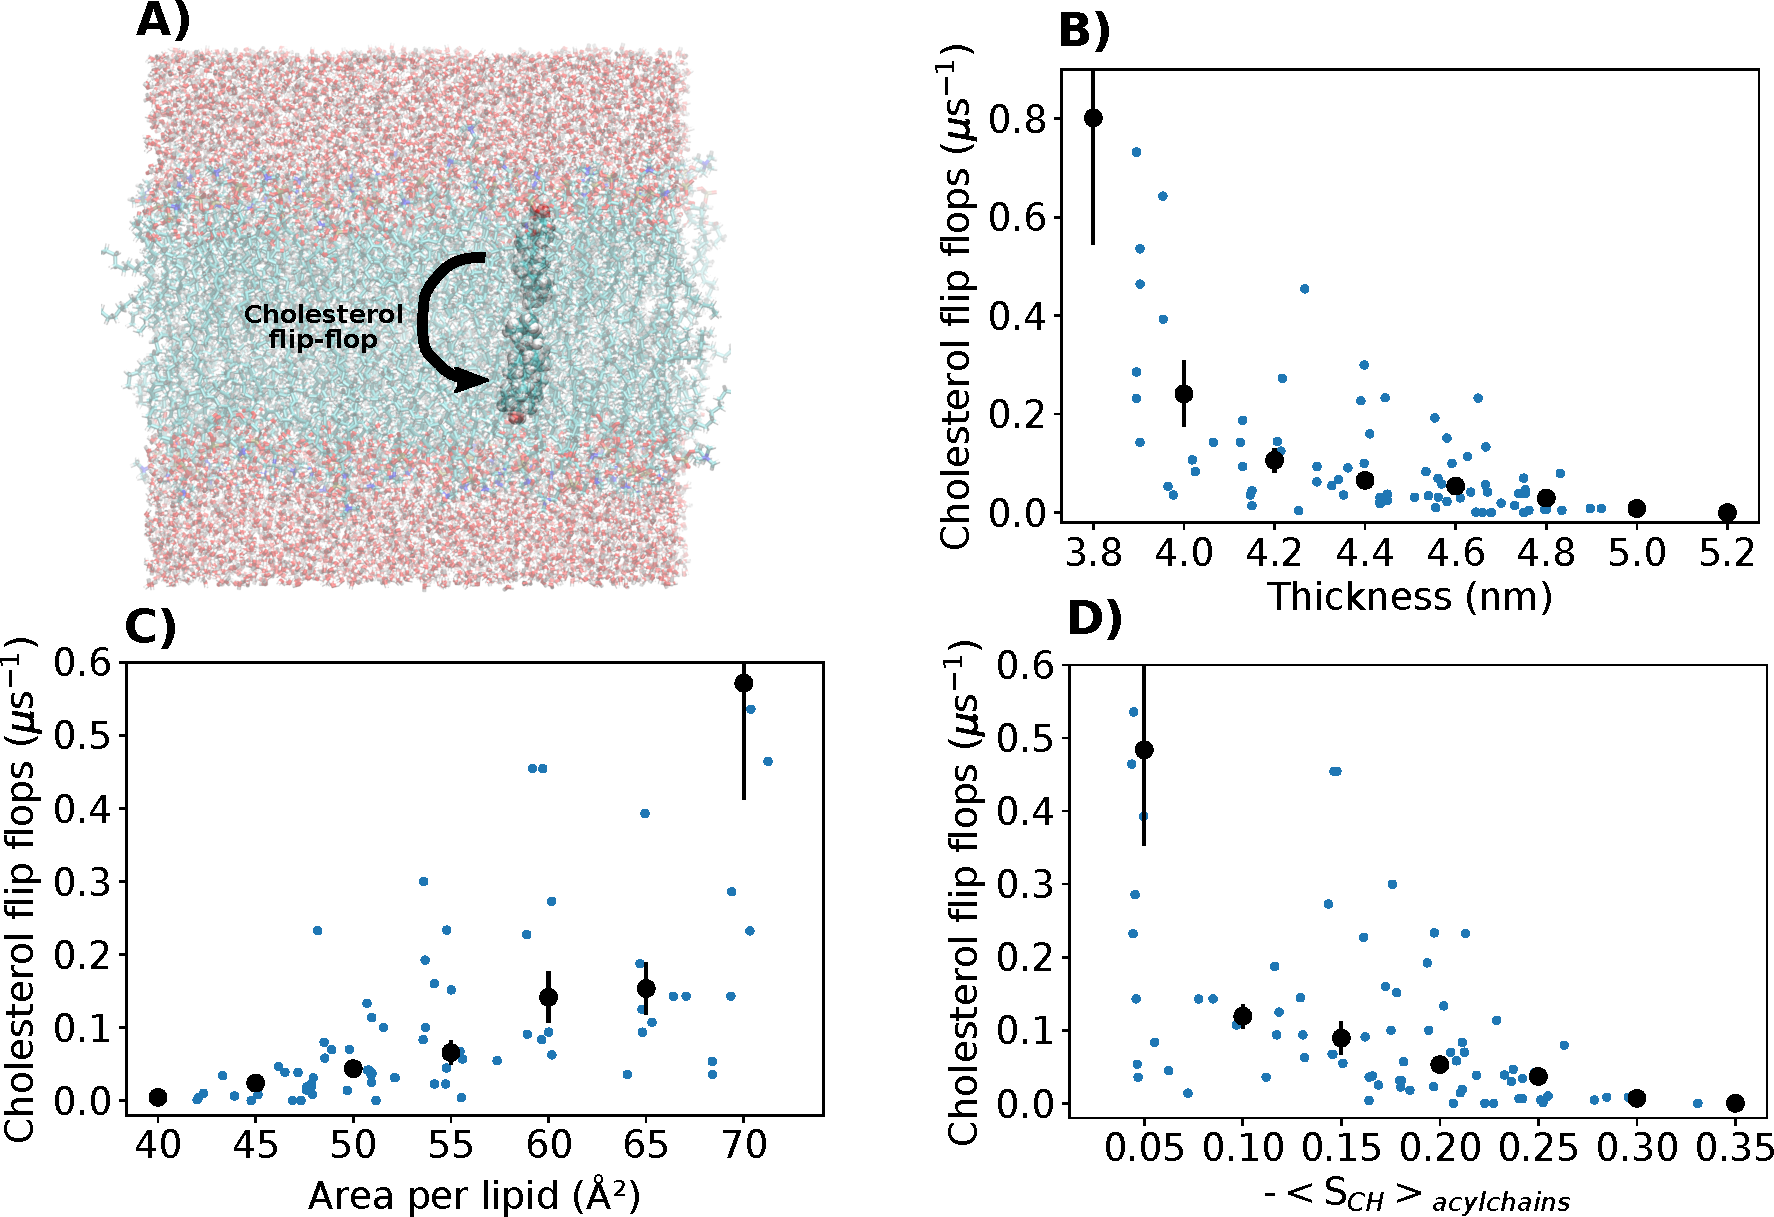
\includegraphics[width=88mm]{Figures/CholFlipFlops.pdf}
    \caption{{\bf A} Illustration of cholesterol flip-flop.  
      {\bf B-D} Cholesterol flip-flops analyzed from the databank as a function of membrane thickness, area per lipid, and acyl chain order. Values from simulations with non-zero flip-flop rates are shown with blue dots. Averages over fixed range of x-axis values are shown with black dots.
    }
    \label{fig:flip-flops}
\end{figure}

MD simulation and exploration of the cholesterol flip-flops phenomenon has only recently become possible for research groups with substantial resources and specialized expertise~\cite{gu19,javanainen19,baral20}. Our analysis demonstrates how the NMRlipids databank makes analyses of such rare phenomena accessible to wide range of scientists in different fields of science and industry who do not have the access to required resources and expertise to produce the large amounts of MD simulation data required. 


\subsection{Extending the scope of MD simulations to new fields using the NMRlipids databank: Water diffusion anisotropy in membrane systems}
The anisotropy in water diffusion in parallel and perpendicular directions with respect to membranes plays a role in the drug translocation through biological material, particularly in skin \cite{hansen13,wen18,nitsche19,roberts21} and in MRI imaging~\cite{topgaard20}. MD simulations are rarely used to analyze anistropic diffusion of water since only few permeation events for water are typically observed in a single MD simulation trajectory~\cite{venable19,camilo2022}, making the collection of sufficient data challenging or impossible. Here, we show that the NMRlipids databank can be used to systematically analyze how anisotropic water diffusion in a multilamellar membrane systems depends on membrane properties. 

\begin{figure}[tb]
    \centering
    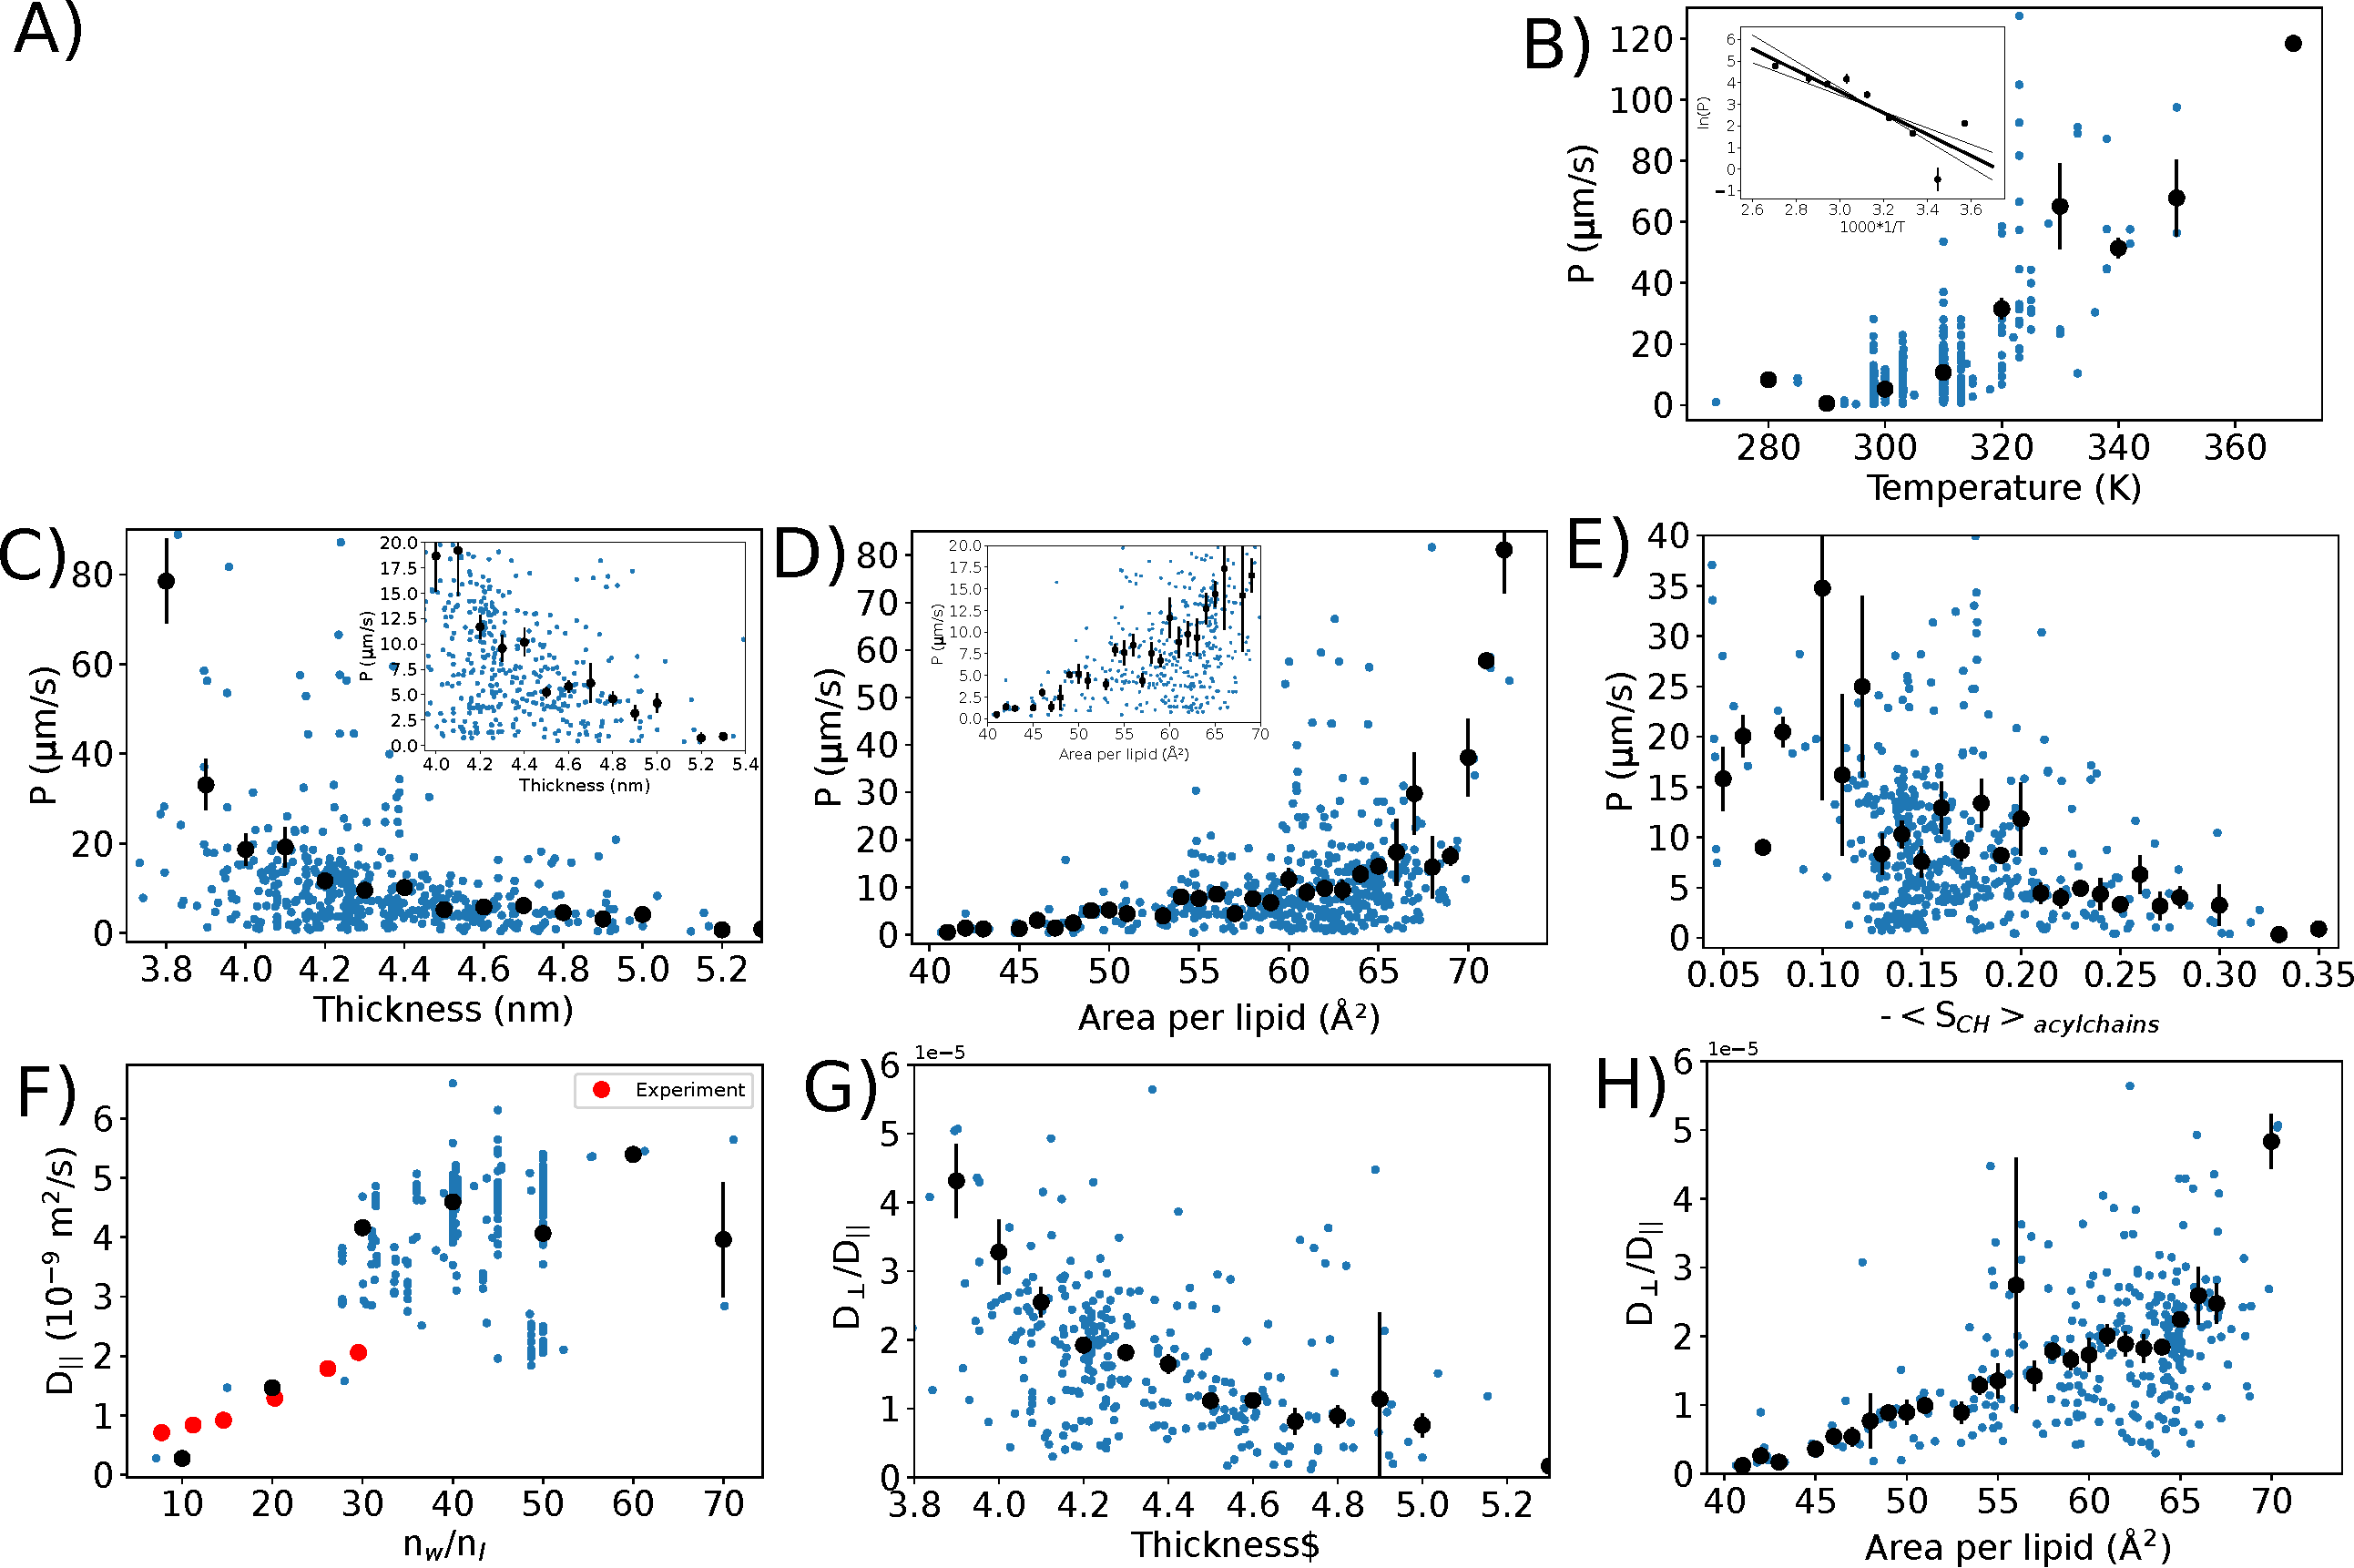
\includegraphics[width=180mm]{Figures/permeation2.pdf}
    \caption{{\bf A} Water diffusion, $D_\perp$, and permeability, $P$, through membranes, and lateral diffusion along the membrane, $D_{||}$, illustrated in a multilamellar stack of lipid bilayers. 
    {\bf B-E} Water permeation through membranes analyzed from the databank as a function of temperature, thickness, area per lipid, and acyl chain order. Values from simulations with non-zero permeation values are shown with blue dots. Averages over fixed range of x-axis values are shown with black dots. Insert in B) shows the Arrhenius plot of permeation ($\ln$ (P) vs. 1/T) that gives 17\,$\pm$\,4\,k$_b$T for the average activation energy for water permeation through lipid bilayer. Inserts in C) and D) show the region where the dependence could be considered approximately linear.
    {\bf F} Lateral diffusion of water as a function of hydration level. Experimental points for DMPC bilayers at 313\,K at different hydration levels are shown~\cite{rudakova04}.
    {\bf G-H} Diffusion anistoropy of water as a function of thickness and area per lipid. }
    \label{fig:permeability}
\end{figure}


To this end, we calculated the water permeability through membranes from all simulations in the NMRlipids databank. The resulting non-zero values range between 0.3 and 322\,$\mu$m/s with a mean and median of 14\,$\mu$m/s and 8\,$\mu$m/s, respectively. These values agree with the previously reported simulation results~\cite{venable19,camilo2022} and have the same order of magnitude as experimentally determined diffusive permeability coefficients, but are on average larger than the values reported for PC lipids in the liquid crystalline phase,~0.19-0.33\,$\mu$m/s~\cite{jansen95}. Observed permeabilities and their averages over fixed ranges of values at $x$-axis are shown in Figs.~\ref{fig:permeability} B-E as a function of temperature, membrane thickness, area per lipid, and acyl chain order.  
%on average, we calculated the average permeabilities over all systems with the value of temperature, thickness, area per lipid, or acyl chain order within a fixed range. These averaged permeabilities also shown in Figs.~\ref{fig:permeability} with black dots. 
As expected, the permeability increases with the temperature, giving an average energy barrier of 17\,$\pm$\,4\,k$_b$T for the water permeation from the Arrhenius plot in Fig.~\ref{fig:permeability} B. On the other hand, the permeability of water decreases on average when membranes become more packed, i.e., with decreasing area per lipid and increasing thickness and acyl chain order (Figs.~\ref{fig:permeability} C-E). Permeation of water through bilayers also depends on membrane properties according previous studies, but there is no established consensus on whether the area per lipid~\cite{nagle08} or bilayer thickness~\cite{frallicciardi22} is the main parameter determining the permeability. 
%is previously reported from simulations and experiments for some systems, but not for all~\cite{mathai07,venable19,frallicciardi22}. 
Our analysis over the NMRlipids databank, containing significantly more data than that was available in previous studies, suggest non-linear dependence on both of these parameters, yet the linear correlation would be a good approximation for thicknesses above $\sim$\,3.9\,nm and area per lipids below $\sim$69\,Å$^2$ (insets in Figs.~\ref{fig:permeability} C-D).
%within the range of experimentally reported values  permeability which is 1-2 orders of magnitude slower than osmotic permeability \cite{jansen95,??}. 
Clear dependencies of permeability on charged lipids, cholesterol, POPE, or hydration level were not observed in Fig.~\ref{fig:permeationSI} in the supplementary information.
%, although weak decrease for the latter two may be visible.
%
%
%
%%Several models on how water dynamics depends on membrane properties have been proposed based on different experimental and %%theoretical methods, yet consensus 
%%%on how water permeability depends on membrane properties, such as area per lipid and thickness, or molecular composition, 
%%has not been reached~\cite{mathai07,nitsche13,nitsche16,shinoda16,venable19,frallicciardi22}.  




To analyze how water diffusion anisotropy depends on membrane properties in a multi-lamellar lipid bilayer system, we calculated the water diffusion parallel to the membrane surface from all simulations in the NMRlipids databank. The parallel diffusion coefficient of water, $D_{||}$, decreases with reduced hydration and increases with the temperature, but dependencies on membrane area per lipid, thickness, or fraction of charged lipids were not observed in Figs.~\ref{fig:permeability} and~\ref{fig:diffusionSI}.
%The experimental water diffusion increases with increasing hydration level toward the value for bulk water . 
%As expected, water translational diffusion increase in the diffusion is observed with the increased temperature and hydration level (Figs.~\ref{fig:permeability} H and~\ref{fig:diffusionSI} B). 
%The results at different hydration levels are shown in Fig.~\ref{fig:permeability} F together with the experimental data~\cite{rudakova04}. 
Simulation results are close to the experimental values with low hydration levels in Fig.~\ref{fig:permeability} F, but increase to approximately two times higher than the experimental value for bulk water diffusion (3.1$\cdot$\,10$^{-9}$\,m$^2$/s at 313\,K~\cite{khakimov08}) with high hydration levels. This is not surprising as the most common water model used in membrane simulations, TIP3P, is known to overestimate the bulk water diffusion~\cite{pathirannahalage21}. To estimate the diffusion anisotropy of water, $D_{\perp}/D_{||}$, in multi-lamellar membrane system, the permeability coeffients of water through membranes were translated to perpendicular diffusion coefficients, $D_{\perp}$, using the Tanner equation~\cite{tanner78,wasterby02}. The resulting perpendicular diffusion coefficients are approximately five orders of magnitude smaller than lateral diffusion coefficients of water (Figs.~\ref{fig:permeability} G and H), which is at the upper limit of the anisotropic diffusion as determined by experiments~\cite{nitsche19}. 
%Large anisotropy values are understandable as simulations give slightly slower permeation rates and higher lateral diffusion rates than experiments. 
Significant increase in the diffusion anisotropy with membrane packing is observed, as $D_{\perp}/D_{||}$ drifts away from one with decreasing area per lipid and increasing thickness in Figs.~\ref{fig:permeability} G and H. This follows from decreasing water permeability with membrane packing (Figs \ref{fig:permeability} C and D), while lateral diffusion remains approximately constant (Fig. \ref{fig:diffusionSI} A and C). 

In conclusion, our results suggest that the bilayer packing has a substantial effect on anisotropic water diffusion in multi-membrane lipid systems. Several folds larger anisotropy in membranes with higher lateral density is expected to play a role in pharmagokinetic models, not only for water but also for other hydrophilic molecules~\cite{nitsche19}. Furthermore, the enhanced understanding of this anisotropy may help in developing new MRI imaging methods~\cite{topgaard20}.

\section{Discussion}

%The Discussion should be succinct and must not contain subheadings.

The focus of biomolecular simulations is moving from studies of individual molecules to larger complexes and even whole cells and organelles~\cite{johnson15,thornburg22,gupta22}. On the other hand, machine learning based models predicting behaviour of biomolecules and automatic approaches to parametrize models are emerging~\cite{jumper21,antila22b}. The NMRlipids databank will support the development in all these directions. The automatic quality evaluation and ranking of simulations in the NMRlipids databank guides the optimization of new force field parameters and the selection of best parameters for large biomolecular complexes where simulation quality becomes increasingly important due the multiplication of small errors in large simulations. On the other hand, the NMRlipids databank serves as a training set for diverse machine learning applications. 
%Most straightforward applications include models that would predict connections between membrane properties that are already stored in the databank. 
For example, a machine learning model predicting electron density profiles from form factors would be highly useful in interpretation of scattering experiments. On the other hand, more elaborated models can be trained to predict arbitrary membrane properties using the data from the NMRlipids databank. 

Providing programmatic access to large scale MD simulation data in the NMRlipids databank can lead to applications in unprecedented directions in fields where MD simulations are less commonly utilized. Here we exemplified this by analysing the anisotropic diffusion of water (Fig.~\ref{fig:permeability}), which is relevant in pharmacokinetic modeling and in MRI imaging where MD simulations are not yet commonly used~\cite{nitsche19,topgaard20}. 
%The NMRlipids databank will be of great benefit to scientists involved in MD simulations. They will be able to rapidly evaluate the quality of MD simulations in order to filter out potentially misleading results or facilitate force field parameter development~\cite{antila22b}. The selection of best models for a specific application is demonstrated for PC/PE lipid mixtures in Fig.~\ref{fig:quality}, and previously for PC/PS lipid mixtures~\cite{antila22b}, and lipid headgroups~\cite{bacle21}. 
On the other hand, programmatic access in the NMRlipids databank enables automatic analyses over larger sets of simulation data in terms of quantity (e.g., simulation length and number of conformations) and content (e.g, lipid compositions and ion concentrations) that is currently possible in a single research group. Added value of such access to simulation data is demonstrated here for the analysis of simulation qualities (Fig.~\ref{fig:quality}), water permeation through membranes (Fig.~\ref{fig:permeability}) and cholesterol flip-flop events (Fig.~\ref{fig:flip-flops}). 
%Such models could be used to connect membrane composition to relevant membrane properties in wide range of fields from molecular biology to drug development and biomolecular imaging. 
Different types of applications enabled by the NMRlipids databank in wide range of fields are exemplified in Table~\ref{tab:applications}. The increasing amount of data is expected to further increase the scope of potential applications of the NMRlipids databank in wide range of fields ranging from molecular biology and biotechnology to
%the design of lipid nanoparticles for drug delivery or other applications, and 
material science and biomolecular imaging. 

\begin{table}[t]
    \centering
    \begin{tabular}{p{5.0cm}  p{5.0cm}  p{4.0cm}}
    Type of application     & Practical examples & Target group \\
    \hline
    Analyses of rare phenomena               & Lipid flip-flops, water permeation & Membrane scientists \\
    \\
    Correlations between membrane properties & 
    Membrane structural properties, water dynamics (Figs.~\ref{fig:quality} and~\ref{fig:permeability}) & 
    Membrane scientists \\
    \\
    Applications that are outside typical scope of MD simulations & 
    Anisotropic water diffusion for pharmagokinetics and MRI imaging applications & 
    Scientist in fields where MD simulations are not usually applied \\
    \\
    Selection of the best simulation model for a specific application & 
    Best model for POPC lipids (Fig.~\ref{fig:quality}), headgroup conformations~\cite{bacle21}, 
    packing of PS~\cite{antila22b} and PE (Fig.~\ref{fig:POPCPOPEapls}) containing membranes. &
    Scientists using MD simulations \\
    \\
    Guidance for force field development & 
    Improvements in ion binding to lipids~\cite{melcr18,melcr20} and lipid headgroup conformational ensembles~\cite{yu21,dickson22,grote20} &
    Scientists developing parameters for MD simulations \\
    \\
    Training and target data for coarse grained models & 
    Optimizing parameters of coarse grained models against NMRlipids databank, extracting continuum parameters for membranes. &
    Scientists developing and using coarse grained MD simulations \\
    \\
    Training set for machine learning applicatons &
    programmatic access to the data and results enables training of machine learning type of models for various applications, such as predictions of membrane properties from composition & Scientists building and using machine learning applications for biomolecules.  
    \end{tabular}
    \caption{Examples on applications of the NMRlipids databank.}
    \label{tab:applications}
\end{table}



Main practical limitations in building open access databanks of molecular dynamics simulations have been the required commitment in long term support for hardware and software maintenance, and the lack of incentives for researchers to share the data. The NMRlipids databank circumvents these challenges with the overlay databank design and open collaboration approach developed in the NMRlipids project~\cite{botan15}. In this model, the file storage is distributed to publicly available stable repositories ({\it Data layer} in Fig.~\ref{fig:overlay} A) and maintenance of the databank does not depend on individual scientists or groups because all its version controlled content is available with an open access licence ({\it Databank layer} in Fig.~\ref{fig:overlay} A). 
%containing relevant information about the trajectories, including the location of the raw data. This architecture streamlines the construction and maintenance of the databank
%
%, the demand of hardware can be distributed and open collaboration model reduces the risk for ending software maintenance. 
%Furthermore, the 
%by distributing the long term commitment for hardware and software maintenance. 
Incentive to share the data is created in the NMRlipids open collaboration by offering authorship in published articles to the contributors following the NMRlipids project protocol~\cite{botan15}.
%, thereby creating an incentive for contributions. 
%
%Universal quality measures and naming conventions for molecules and atoms are defined in the NMRlipids databank to enable the automatic quality evaluation and other analyses.
%
%of lipid bilayer MD simulations introduced in the NMRlipids databank enables rapid ranking of available simulation models agains experimental NMR and x-ray scattering data. 
%
The current NMRlipids databank contains only lipid bilayer simulations, but the concept can be applied also to other biomolecules, such as disordered proteins and membrane-protein systems,
%combining open collaboration and overlay databank structure can be applied also 
or other fields where similar barriers to establish publicly accessible databanks exist. 
%The overlay databank design can open such avenues also for other 

%
%, thereby not requiring large resources to handle and maintain. 
%This lowers the barrier for starting such databank as well as for long term storage. 
%The NMRlipids databank  
%In addition to all computers where the databank is developed and used, the NMRlipids databank git is stored to Zenodo server, thereby enabling a very cost effective long term storage for the databank. 


\newpage


\section{Methods}

%Topical subheadings are allowed. Authors must ensure that their Methods section includes adequate experimental and characterization data necessary for others in the field to reproduce their work.

\subsection{Structure of the databank}
Structure of the NMRlipids databank is illustrated more detailed in Fig.~\ref{DatabankStructure} in the supplementary information. The core content of the databank ({\it Databank layer} in Fig.~\ref{fig:overlay}) locates as a git repository at \url{https://github.com/NMRLipids/Databank/} and is permanently stored in Zenodo repository (\url{www.zenodo.org})~\cite{??}. Whenever a specific file is referred here, the file path within the NMRlipids databank repository is given. The scripts in the NMRlipids databank are mainly written in Python and many of them utilize the MDAnalysis module~\cite{gowers2019mdanalysis,michaud2011mdanalysis}.

Essential information of each simulation in the NMRlipids databank is stored in a human and machine readable README.yaml file located at {\it /Data/Simulations} in the NMRlipids databank repository. These files contain access to all information that are needed for further analyses of simulations. The content of these files is described in detail in table~\ref{tab:READMEkeys} in the supplementary information. 
%To keep the databank light, 
Raw MD simulation data are stored in external publicly available and stable repositories ({\it Data layer} in Fig.~\ref{fig:overlay}), such as Zenodo (\url{www.zenodo.org}), from where it can be downloaded whenever needed using the links in README.yaml files.  


\subsection{Molecule and atom naming convention} \label{naming}
When analysing simulations, atoms and molecules needs to be often called by their names defined in the simulation trajectory. However, these names typically vary between force fields because the universal naming convention has not been defined for lipids. To enable automatic analyses over simulations with different atom and molecule names in the NMRlipids databank, we have defined unique naming conventions for molecules and atoms therein. Unique abbreviations used in the NMRlipids databank for each molecule are listed in table~\ref{tab:abbreviations} in the supplementary information. Atom names used in simulation trajectories are connected to unique atom names using mapping files that are defined in the NMRlipids project (\url{https://nmrlipids.blogspot.com/2022/04/new-yaml-format-of-mapping-files.html}). These files are located at {\it /Scripts/BuildDatabank/mapping\_files} in the NMRlipids databank repository. These files also define whether an atom belongs to headgroup, glycerol backbone, or acyl chain region in a lipid. In practise, force field specific molecule names and mapping files
names are given in the COMPOSITION dictionary in README.yaml files for each molecule in each simulation in the NMRlipids databank.

\subsection{Adding data into the NMRlipids databank}
The NMRlipids databank is open for additions of simulation data by anyone. The first step is to create an info.yaml file containing the information that needs to be manually entered as listed in table~\ref{tab:READMEkeys}. This file can be then added into {\it /Scripts/BuildDatabank/info\_files} folder in the NMRlipids databank repository via pull requests. After the pull request is manually accepted, the rest of the information for the README.yaml file, listed in table~\ref{tab:READMEkeys}, will be automatically extracted using the {\it /Scripts/BuildDatabank/AddData.py} script. Currently the NMRlipids databank is composed of simulations found from Zenodo repository with an appropriate licence. Most, but not all, of these trajectories originate from previous NMRlipids projects~\cite{botan15,catte16,antila19,bacle21}.

\subsection{Experimental data}
Experimental data used in the quality evaluation, currently composed of C-H bond order parameters and x-ray scattering form factors, are stored in {\it /Data/experiments} in the NMRlipids databank repository. Similarly to simulations, each experimental data set has a README.yaml file containing all the relevant information about the experiment. The keys and their descriptions for the experimental data are given in table~\ref{tab:READMEkeysEXP}. NMR data currently in the NMRlipids databank are taken from Refs.~\citenum{scherer87,ferreira13,antila19,melcr20,bacle21} and x-ray scattering data from Refs.~\citenum{Kucerka08a,kucerka11,pan12b,pan14,kucerka15}. In addition, some previously unpublished NMR and x-ray scattering data are used. These are measured with previously established methods as described in the supplementary information. 

\subsection{Analyzing the databank}
Programs that analyze large data sets from the NMRlipids databank loop over README.yaml files of all simulations, download the raw simulation data to the local computer, and perform the analysis from the downloaded trajectories. When molecule or atom names are needed in the analysis, they will be read from the README.yaml file and mapping files defined therein.

\subsection{Calculation of C-H bond order parameters}
The C--H bond order parameters were calculated directly from the carbon and hydrogen positions using the definition
%The order parameters are defined as
\begin{equation}\label{OP}
S_{\rm CH}=\frac{1}{2}\left\langle 3\cos^2\theta -1 \right\rangle,
\end{equation}
where angular brackets denote the ensemble average, i.e., average over all sampled configurations of all lipids in a simulation, and $\theta$ is the angle between the C--H bond and the membrane normal. As in previous NMRlipids publications, the order parameters were first calculated separately for each lipid and the standard error of the mean over different lipids was used as the error bar~\cite{botan15}. The script that calculates C-H bond order parameters from all simulations in the NMRlipids databank is available at {\it /Scripts/AnalyzeDatabank/calcOrderParameters.py} in the NMRlipids databank repository. The resulting order parameters are stored for all simulations in files named %\newline 
[{\it lipid\_name}]{\it OrderParameters.json} at folders in {\it /Data/Simulations} in the NMRlipids databank repository.

\subsection{Calculation of x-ray scattering form factors}
X-ray scattering form factors were calculated with standard equation for symmetric lipid bilayers~\cite{ollila16}
\begin{equation}\label{FFsimpl}
F(q)=\int_{-D/2}^{D/2}\Delta \rho_e(z) \cos(zq_z) {\rm d}z,
\end{equation}
where $\Delta \rho_e(z)$ is the difference between total and solvent electron densities, and $D$ is the simulation box size in the z-direction. For the calculation of density profiles, atom coordinates were first centred around the centre of mass of lipid molecules for every time frame, and a histogram of these centred positions weighted with the number of electrons in each atom was then calculated with the bin width of $1/3$~Å. 
%Similarly to order parameters, the script loops over all simulations, downloads the data on local computer, and uses the information in README.yaml file to calculate form factors. 
The script to calculate form factors for all simulations in the NMRlipids databank is available at {\it Scripts/AnalyzeDatabank/calc\_FormFactors.py}. The resulting form factors are stored for all simulations in files named {\it FormFactor.json} at folders in {\it /Data/Simulations} in the NMRlipids databank repository.

\subsection{Calculation of a bilayer area per lipid and thickness}
Area per lipids of bilayers were calculated by dividing the area of the simulation box with the total number of lipid molecules in the simulation. The script that calculates area per lipids from all simulations in the NMRlipids databank repository is available at {\it Scripts/AnalyzeDatabank/calcAPL.py} in the NMRlipids databank repository. The resulting area per lipids are stored for all simulations in files named {\it apl.json} at folders in {\it /Data/Simulations}. 

Thicknesses of lipid bilayers were calculated from the intersections of lipid and water electron densities. The script that calculates thickness of all simulations in the NMRlipids databank is available at {\it Scripts/AnalyzeDatabank/calc\_thickness.py} in the NMRlipids databank repository. The resulting thicknesses are stored in files named {\it thickness.json} at folders in {\it /Data/Simulations} in the NMRlipids databank repository. 

\subsection{Quality evaluation of C-H bond order parameters}
As the first step to evaluate simulation qualities against experimental data, each simulation is connected to an experimental data if molar concentrations of all molecules are within $\pm$3 percentage units, charged lipids have the same counterions, and temperatures are within $\pm$2 degrees. For molar concentrations of water, the exact hydration level is considered only for systems with molar water to lipid ratio below 25, otherwise the systems are considered as fully hydrated. In practise, this is implemented by adding the path of the experimental data into the simulation README.yaml file using the {\it /Scripts/BuildDatabank/searchDATABANK.py} script in the NMRlipids databank repository. 

%\subsubsection{Conformational ensembles using C-H bond order parameters}
%
%The quality of conformational ensembles of individual lipid molecules in simulations are evaluated using the C-H bond order parameters which can be directly compared with robust experimental data~\cite{ollila16}.

The quality of each C--H bond order parameter is estimated by calculating the probability for a simulated value to locate within the error bars of the experimental value. Because conformational ensembles of individual lipids are independent in a fluid lipid bilayer, $\frac{S_{\rm CH}-\mu}{s/\sqrt{n}}$ has a Student's t-distribution with $n-1$ degrees of freedom, and the probability for an order parameter from simulation to locate within experimental error bars can be estimated from equation
\begin{equation}\label{probability}
  P = f \left( \frac{S_{\rm CH} - (S_{\rm exp}+\Delta S_{\rm exp})}{s/\sqrt{n}} \right) - f \left( \frac{S_{\rm CH} - (S_{\rm exp}-\Delta S_{\rm exp})}{s/\sqrt{n}} \right),
\end{equation}
where f(t) is the %first order 
Student's t-distribution, $\mu$ is the real mean of the order parameter, $n$ is the number of independent sample points for each C-H bond which equals the number of lipids in a simulation, $S_{\rm CH}$ is the sample mean from Eq.~\ref{OP}, $s$ is the variance of $S_{\rm CH}$ calculated over individual lipids, $S_{\rm exp}$ is the experimental value, and $\Delta S_{\rm exp}$ its error. The error of $\Delta S_{\rm exp} = 0.02$ is currently assumed for all experimental order parameters~\cite{ollila16}, yet more accurate may be available in the future~\cite{wurl22}. Because a lipid bilayer simulation contains at least dozens of lipids, the Student's t-distribution could be safely approximated with a normal distribution. However, the normal distribution gives probability values that are below the numerical accuracy of computers when simulation values are far from experiments. To avoid such numerical instabilities, we use the first order Student's t-distribution having slightly higher probabilities for values far away from the mean.
%Because phospholipids sample their conformational ensemble within nanosecond timescale~\cite{ferreira15}, all simulations in the databank would be sufficiently long to sample the realistic conformational phase of individual lipids. 
On the other hand, some force fields exhibit too slow dynamics which leads to large error bars in order parameter values~\cite{antila21a}. Such large error bars widen the Student's t-distribution in Eq.~\ref{probability} thereby artificially increasing the probability to find the simulated value within experimental error bars. Therefore, the order parameters with simulation error bars above the experimental error 0.02 are not included in the quality evaluation.



%We estimate the probability for the simulation order parameter to locate within experimental
%error bars from equation
%\begin{equation}\label{probability}
%  P = T(S_{\rm exp}+\Delta S_{\rm exp}) - T(S_{\rm exp}-\Delta S_{\rm exp}),
%\end{equation}
%where T is the first order Student's t-distribution shifted to $\bar{X}$ and
%scaled with $s$. 
%where the probability is calculated from the normal distribution
%\begin{equation}\label{gaussian}
%    P = \int_{S_{\rm exp}-\Delta S_{\rm exp}}^{S_{\rm exp}+
%    \Delta S_{\rm exp}}  \frac{1}{\sigma \sqrt{2\pi}} e^{-\frac{1}{2}(\frac{x-\mu}{\sigma})^2} {\rm d}x.
%\end{equation}
%$S_{\rm exp}$ and $\Delta S_{\rm exp}$ are experimental order parameter and its error, and $\mu$ and $\sigma$ are the mean order parameter and its standard deviation from simulations. The quality measure $S_q$ approaches to zero when probability for agreement between simulation and experimental results approach one, and increases when simulated and experimental values diverge.

To streamline the comparison between simulations, we define the qualities of different fragments (headgroup, acyl chains or total lipid) within each lipid type in a simulation as
\begin{equation}
    P^{\rm frag}[{\rm lipid}] = \frac{\langle P[{\rm lipid}]\rangle_{\rm frag}}{p_{\rm frag}[{\rm lipid}]},
\end{equation}
where $\langle P[{\rm lipid}]\rangle_{\rm frag}$ is the average of individual C-H bond order parameters qualities within the fragment, $p_{\rm frag}[{\rm lipid}]$ is the percentage of order parameters for which the quality is available within the fragment, and frag can be {\it sn}-1, {\it sn}-2, headgroup or total (all order parameters within a molecule). The overall quality of different fragments in a simulation are then defined as a molar fraction weighted average over different lipid components
\begin{equation}
    P^{\rm frag} = \sum_{\rm lipid} \chi_{\rm lipid} P^{\rm frag}[{\rm lipid}],
\end{equation}
where $\chi_{\rm lipid}$ is the molar fraction of a lipid in the bilayer.

The quality evaluation of order parameters is implemented in {\it /Scripts/BuildDatabank/QualityEvaluation.py} in the NMRlipids databank repository. The resulting qualities for each order parameters are stored in files named  [{\it lipid\_name}]{\it \_OrderParameters\_quality.json}, for individual lipids in files named [{\it lipid\_name}]{\it \_FragmentQuality.json}, and for overall quality for fragments in files named {\it system\_quality.json} at folders in {\it /Data/Simulations} in the NMRlipids databank repository. 


\subsection{Quality evaluation of x-ray scattering form factors}
%While C-H bond order parameters relate to the conformational ensembles of individual lipids, the x-ray scattering form factors depend on membrane dimensions and density distribution~\cite{ollila16}.
Because experiments give form factors only in relative intensity scale, they should scaled before comparing with the simulation data. Here we use the scaling coefficient for experimental intensities defined in the SIMtoEXP program~\cite{kucerka10}
\begin{equation}
    k_e = \frac{\sum_{i=1}^{N_q} \frac{|F_s(q_i)||F_e(q_i)|}{(\Delta F_e(q_i))^2}}{\sum_{i=1}^{N_q} \frac{|F_e(q_i)|^2}{(\Delta F_e(q_i))^2}},
\end{equation}
%The quality of each form factor was then calculated from the equation
%\begin{equation}
%    \chi^2 = \frac{\sqrt{\sum_{i=1}^{N_q}(|F_s(q_i)|-k_e|F_e(q_i)|)^2/(\Delta F_e(q_i))^2}}{\sqrt{N_q-1}},
%\end{equation}
where $F_s(q)$ and $F_e(q)$ are form factors from a simulation and experiment, respectively, $\Delta F_e(q)$ is the error of the experimental form factor, and summation goes over the experimentally available $N_q$ points. 

Also a quality measure based on differences in simulated and experimental form factors accross available q-range is defined in the SIMtoEXP program~\cite{kucerka10}. However, the lobe heigths in simulated form factors depend on the simulation box size as shown in Fig.~\ref{fig:sizedependence}. Therefore, the quality measure defined in SIMtoEXP  would also depend on the simulation box size. Nevertheless, locations of form factor minima are independent on simulation box size in Fig.~\ref{fig:sizedependence}. Here we use the location of the first form factor minima for the quality evaluation because automatic detection of the location of second minima is inaccurate for some experimental data due to fluctuations, such as for the POPE data in Figs.~\ref{fig:quality} D and E. 
%In order to define a quality measure which is independent on simulation box size, we measure the form factor quality based on the location of the first minima observed in experiments. 
The first minimum correlates well with the thickness of a membrane (Fig.~\ref{fig:quality} F), although the correlation of the second minima would be even stronger (Fig.~\ref{fig:QualityCorrelationsSI}). In practise, we first filter the fluctuations from the form factor data using Savitzky-Golay filter (window lenght 30 and polynomial order 1) and locate the first minima above 0.1\,\AA$^{-1}$ from both simulation and experimental data. The quality of a form factor is then defined as Eucledian distance between the minima in simulated and experimental form factors, $FF_q = |FF_{\rm{min}}^{\rm{sim}}-FF_{\rm{min}}^{\rm{exp}}|$. 

The quality evaluation of form factors is implemented in {\it /Scripts/BuildDatabank/QualityEvaluation.py} in the NMRlipids databank repository. The resulting form factor qualities are stored in files named {\it FormFactorQuality.json} at folders in {\it /Data/Simulations} in the NMRlipids databank repository.


\subsection{Calculation of lipid flip-flops}
Flip-flop rates were calculated using {\it AssignLeaflets} and {\it FlipFlop} tools from LiPyphilic package~\cite{LiPyphilic2021}. Headgroup atoms of each molecule as defined in the mapping file were used to determine in which leaflet the molecule locates. The midplane cut-off defining the region between leaflets was 1\,nm and frame cut-off was 100. This means that if the headgroup of a molecule entered within the distance of 1\,nm from the bilayer midplane and was found from the opposing leaflet after 100 steps, this event was considered as a successfull flip-flop event. The code that finds flip-flop events from all simulations in the NMRlipids databank is available at {\it scripts/FlipFlop.py} and the results at {\it Data/Flipflops/} in the repository at~\url{https://github.com/NMRLipids/DataBankManuscript/}. 


\subsection{Analysing anisotropic diffusion of water in membrane environment from the NMRlipids databank}

%The README.yaml files contain all the essential information to perform arbitrary analyses of simulations in the NMRlipids databank, i.e., the permanent location of the original data and naming convention for all atoms and molecules in each system. 
%In practise, the analyse codes contains a loop over all README.yaml files (i.e., simulations in the NMRlipids databank) which first downloads the raw simulation to a local computer and then uses the information about the atom and molecule naming conventions in README.yaml and mapping files to perform the desired analyses. 

%A minimal example of a analysis code is available at \url{https://github.com/NMRLipids/Databank/blob/main/Scripts/AnalyzeDatabank/template.ipynb}.

Water permeability through membranes was calculated from equation $P=r/2c_w$, where $r$ is the rate of permeation events per time and area, and $c_w$=33.3679\,(nm)$^{-3}$ is the concentration of water in bulk~\cite{venable19}. The number of permeation events in each trajectory was calculated using the code by Camilo et al.~\cite{camilo2022}, available at~\url{https://github.com/crobertocamilo/MD-permeation}. 
%This code was used within the loop that goes over all simulations in the NMRlipids databank and extracts the required information using the information in README.yaml files. 
The code that calculates permeabilities for all simulations in the NMRlipids databank is available at {\it /scripts/calcMD-PERMEATION.py} and the resulting permeabilities are stored at {\it /Data/MD-PERMEATION} in the repository containing all analyses specific for this publication at~\url{https://github.com/NMRLipids/DataBankManuscript/}. 
%While the order parameters, form factors, area per lipid and thickness are stored within the NMRlipids databank (\url{https://github.com/NMRLipids/Databank/tree/main/Data/Simulations}), further analyses can be conventiently stored in separate repositories with the same folder structure based on hash identities of trajectory and topology files. For example, results from further analyses performed here are stored in folders at \url{https://github.com/NMRLipids/DataBankManuscript/tree/main/Data}. 
This repository is organized similarly to the NMRlipids databank repository, enabling the upcycling of also the analyzed data without overloading the main NMRlipids databank repository. 

The lateral diffusion of water along the membrane surface, $D_{||}$, was calculated with Einstein's equation using {\it -lateral} option in {\it gmx msd} program within the Gromacs software package~\cite{gromacsMANUAL}. The code that calculates $D_{||}$ for water from all simulations in the NMRlipids databank is available at {\it /scripts/calcWATERdiffusion.py}, and the resulting diffusion coefficients are stored at {\it /Data/WATERdiffusion} in the repository at~\url{https://github.com/NMRLipids/DataBankManuscript/}.

Water diffusion in the perpendicular direction of lipid bilayers in a multilamellar stack was estimated from the Tanner equation $D_\perp = \frac{D_{||} P z_w}{D_{||} + P z_w}$~\cite{tanner78,wasterby02}, where the water layer thickness, $z_w$, was estimated by subtracting bilayer thickness from the size of the simulation box in membrane normal direction.


%\newline \\
%The purpose of a mapping file is to circumvent the problem caused by different atom naming conventions used by different force fields. The first column of a mapping file contains general atom names. The second column contains the name of the atom as it is in the force field. If the lipid consists of several residues which is the case in some AMBER force fields, then a third column is needed which contains the name of the residue to which each atom belongs to.




\bibliography{refs.bib}

%\noindent LaTeX formats citations and references automatically using the bibliography records in your .bib file, which you can edit via the project menu. Use the cite command for an inline citation, e.g.  \cite{Hao:gidmaps:2014}.

%For data citations of datasets uploaded to e.g. \emph{figshare}, please use the \verb|howpublished| option in the bib entry to specify the platform and the link, as in the \verb|Hao:gidmaps:2014| example in the sample bibliography file.

\section*{Acknowledgements}

%Acknowledgements should be brief, and should not include thanks to anonymous referees and editors, or effusive comments. Grant or contribution numbers may be acknowledged.

\section*{Author contributions statement}

Must include all authors, identified by initials, for example:
A.A. conceived the experiment(s),  A.A. and B.A. conducted the experiment(s), C.A. and D.A. analysed the results.  All authors reviewed the manuscript. 

\section*{Additional information}

%To include, in this order: \textbf{Accession codes} (where applicable); \textbf{Competing interests} (mandatory statement). 

%The corresponding author is responsible for submitting a \href{http://www.nature.com/srep/policies/index.html#competing}{competing interests statement} on behalf of all authors of the paper. This statement must be included in the submitted article file.

%\begin{figure}[ht]
%\centering
%
\includegraphics[width=\linewidth]{stream}
%%\caption{Legend (350 words max). Example legend text.}
%\label{fig:stream}
%\end{figure}

%\begin{table}[ht]
%\centering
%\begin{tabular}{|l|l|l|}
%\hline
%Condition & n & p \\
%\hline
%A & 5 & 0.1 \\
%\hline
%B & 10 & 0.01 \\
%\hline
%\end{tabular}
%\caption{\label{tab:example}Legend (350 words max). Example legend text.}
%\end{table}

%Figures and tables can be referenced in LaTeX using the ref command, e.g. Figure \ref{fig:stream} and Table \ref{tab:example}.

\end{document}
